
\documentclass[12pt]{article}
\usepackage[a4paper, total={6.5in, 9in}]{geometry}
\usepackage{import}

\import{./}{macros}


\title{
    % UW Mech/Tron Eng Logo
    
\includegraphics[width=\linewidth]{resources/uwaterloo_mechanical_and_mechatronics_engineering/UWaterloo_Mechanical_and_Mechatronics_Engineering/PNG/UWaterloo_Mechanical_Mechatronics_Eng_Logo_horiz_rgb.png}
    \\[1cm]
    \underline{\bf{ME 212 Billards Project Report}}
}
\author{
    Alex Roman\\
    Austin W. Milne
}
\date{July 17, 2021}


\begin{document}
\maketitle
\vfill
\begin{abstract}
    Project report for ME 212 in Spring 2021. Using MatLab to simulation collisions of pool balls accounting for friction and restitution. Collision videos available \underline{\href{https://uofwaterloo-my.sharepoint.com/:f:/g/personal/awbmilne_uwaterloo_ca/EiWN90NLaUVGpE0EcLgVf8wBgqZj-v4eaprjO5gxFSzF4A?e=SygQLX}{Here}}.
\end{abstract}
\newpage

\tableofcontents
\listoftables
\listoffigures
\lstlistoflistings

\newpage

% \begin{abstract}
% Report 
% \end{abstract}

\section{Part 1 - Collision of 2 Balls}
\subsection{Given Information}
The given problem is to solve for the final velocities of 2 balls with arbitrary mass and initial velocity after colliding at a certain offset distance. Figure \ref{P1_diag} shows the setup of the 2 balls for the collision.

\begin{figure}[H]
    \centering
    \includestandalone[width=10cm]{resources/tikz/part_1_diagram}
    \captionof{figure}{Part 1 Setup}\label{P1_diag}
\end{figure}

\subsection{Physics of The Collision}

Since it can be assumed that there are no external forces during the collision, the problem becomes a straightforward conservation of momentum problem. The velocites can be split for each ball into the direction normal and tangent to the collision. Each part can be solved seperately. First, create a system of equations for the normal velocites before and after the impact. Equations \ref{eqn:pt1_momentum} and \ref{eqn:pt1_restitution} show the equations for conservation of momentum and for impact restitution, respectively.

\begin{equation}
    \label{eqn:pt1_momentum}
    v_a m_a + v_b m_b = v_a' m_a + v_b' m_b
\end{equation}

\begin{equation}
    \label{eqn:pt1_restitution}
    e_{\text{rest.}} = \frac{v_a' - v_b'}{v_b - v_a}
\end{equation}

Solving this system of equations gives the normal velocities of the 2 balls after the collision, $v_a'$ and $v_b'$. For tangent velocities, due to friction, energy loses need to be accounted for in the collision. Since the change in momentum in the normal direction is the intergal of the force over the impact time, the change in tangent velocity can be derived from the change in normal momentum. Equation \ref{eqn:tangent_fric} shows the derivation for a balls tangent velocity after impact.

\begin{equation}
    \label{eqn:tangent_fric}
    \begin{aligned}
        mv + \int_{t_1}^{t_2} Fdt &= mv' \\
        mv_t + \int_{t_1}^{t_2} F_f dt &= mv_t' \\
        mv_t + \mu\left(mv_n' - mv_n\right) &= mv_t' \ \Leftarrow \text{Using $F_f = \mu_k F_n$}\\
        v_t + \mu\left(v_n' - v_n\right) &= v_t'
    \end{aligned}
\end{equation}

\subsection{Application of Physics}
In order to apply the equations above, the normal and tangent velocities of the balls need to be determined. Basic trigonometery can be used to determine the relative velocities. In this case, it is difficult to determine the normal and tangent values from the velocity vector and the $e$ value alone. To make it easier, Figure \ref{P1_diag_exp} shows construction lines added for easier computation.

\begin{figure}[H]
    \centering
    \includestandalone[width=10cm]{resources/tikz/part_1_diagram_expanded}
    \captionof{figure}{Part 1 Construction Lines}\label{P1_diag_exp}
\end{figure}

Using the construction lines above, the below equations can be derived for the tangent and normal velocities of the moving ball. Equation \ref{eqn:part_1_thetas} shows the derivation of the impact angle and relative angles for vector rotation.

\begin{equation}
    \label{eqn:part_1_thetas}
    \begin{gathered}
        h = 2r \\
        \theta = \sin^{-1} \left(\frac{e}{h}\right) = \sin^{-1} \left(\frac{e}{2r}\right)\\
        \theta_\text{velocity} = \tan^{-1}\left(\frac{v_x}{v_y}\right)\\
        \theta_\text{impact} = \theta_\text{velocity} - \theta =  \tan^{-1}\left(\frac{v_x}{v_y}\right) - \sin^{-1} \left(\frac{e}{2r}\right)\\
    \end{gathered}
\end{equation}

Equation \ref{eqn:part_1_impact_v} shows the derivation for the normal and tangent velocities relative to the collision by way of matrix-based vector rotation.

\begin{equation}
    \label{eqn:part_1_impact_v}
    \begin{gathered}
        \phi = \theta_\text{impact} - \theta_\text{velocity}\\
        R = 
        \left[
        \begin{matrix}
            \cos(\phi) & -\sin{\phi}\\
            \sin(\phi) & \cos(\phi)\\
        \end{matrix}
        \right]\\
        v_{a_\text{norm,tang}} = R \times v_a
    \end{gathered}
\end{equation}

Having the normal and tangent velocities for the collision, the below set Equation set \ref{eqn:part_1_together} can be applied to get the final normal and tangent velocities for the both ball A (red) and ball b (white).

\begin{equation}
    \label{eqn:part_1_together}
    \begin{gathered}
        v_{a_n} m_a + v_{b_n} m_b = v_{a_n}' m_a + v_{b_n}' m_b\\
        e_\text{rest.} = \frac{v_{a_n}' - v_{b_n}'}{v_{b_n} - v_{a_b}}\\
        v_{a_t}' = v_{a_t} + \mu \left(v_{a_n}' - v_{a_n}\right)\\
        v_{b_t}' = v_{b_t} + \mu \left(v_{b_n}' - v_{b_n}\right)
    \end{gathered}
\end{equation}

Finally, to get the final velocities of the 2 balls in the $x$-$y$ reference plane, another vector rotation needs to be done to revert to the $xy$ coordinate system. Equation \ref{eqn:part_1_rotate_back} shows this vector rotation.

\begin{equation}
    \label{eqn:part_1_rotate_back}
    \begin{gathered}
        \phi = \theta_\text{velocity} - \theta_\text{impact}\\
        R = 
        \left[
        \begin{matrix}
            \cos(\phi) & -\sin{\phi}\\
            \sin(\phi) & \cos(\phi)\\
        \end{matrix}
        \right]\\
        v_a = R \times v_{a_\text{norm,tang}} \\
        v_b = R \times v_{b_\text{norm,tang}}
    \end{gathered}
\end{equation}


\section{Part 2 - Collisions of a Table of Balls}
\subsection{Given Information}\label{Pt2_Given}
The problem is given to simulate the motion of a set of 11 balls in a square enclosure, Similair to that of a billiards table. The initial position and velocity for each of the balls is provided, along with the mass and radius. Simplifications are made to assume that the system is effectively 2D without spin or rotation. Restitution coefficients for ball-on-ball and ball-on-wall are provided, as well as the frictional coefficient for ball-on-surface, ball-on-wall, and ball-on-ball. Figure \ref{P2_diag} is provided as an example for the visualization of the balls and table.

\begin{figure}[H]
    \centering
    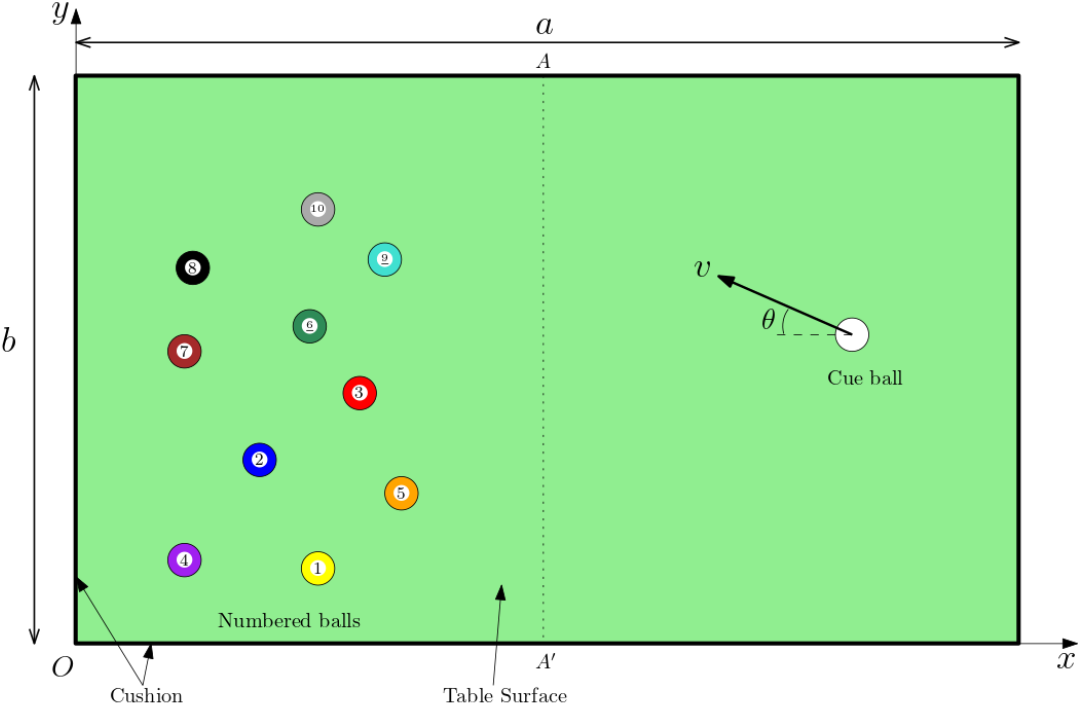
\includegraphics[width=12cm]{resources/Part_2_layout.png}
    \captionof{figure}{Part 2 Table Layout}\label{P2_diag}
\end{figure}

\subsection{Indentifying Collisions and Physics}

In order to simulate the motion of the balls, the different motion states of the balls need to be identified. For balls on a table with bumpers, as outlined in section \ref{Pt2_Given}, there are 3 primary motions: movement for a balls velocity, impact of ball into a wall, and impact of a ball into another ball. Each of these types of motion can be modelled seperately. The strategy used to handle time scales and determine collisions of balls was to calculate the positions of all the balls after very small time changes. After each time interval, each ball is checked for positional overlap with walls and all the other balls on the table. If a ball is overlapping with a wall or another ball, the change in velocity is calculated for the collision. A couple assumptions are made in order to model the system this way. The first assumption is that collisions are instantaneous, and therefore do not have a time range of occurance. This leads to the post-collision velocities being applied instantaneously after balls are determined to be impacting a ball or wall. The second assumption is that the accuracy of using very small time chunks is sufficient enough for the purposes of this simulation. This assumption is substantiated by the calculations in Equation \ref{eqn:part_2_accuracy} which shows that, in the worst case of a glancing shot with maximum time error, the anglular inaccuracy of a collision calculation is equal to roughly 1 millimeter radial displacment over a 2 meter distance.

\begin{equation}
    \label{eqn:part_2_accuracy}
    \begin{gathered}
        \theta_\text{error}^\text{max} = \tan^{-1}\left( \frac{4 \left[\frac{m}{sec}\right] * 
                                         39.3701 \left[\frac{in}{sec}/\frac{m}{sec}\right] *
                                         \frac{1}{100000} \left[sec\right]}{2.25 \left[in\right]} =
                                         0.040102^{\circ}\right)\\
        \sin(\theta_\text{error}^\text{max}) * 2 \left[m\right] = 0.0013998 \left[m\right] = 1.3998 \left[mm\right]
    \end{gathered}
\end{equation}

The equation for 2 balls colliding is already derived and shown in Equation \ref{eqn:part_1_impact_v}, \ref{eqn:part_1_together}, and \ref{eqn:part_1_rotate_back} above. Equation \ref{eqn:part_2_wall} below is the derivation for the velocities after a ball has impacted a wall.

\begin{equation}
    \label{eqn:part_2_wall}
    \begin{gathered}
        v_n' = - e_\text{rest.} v_n \\
        v_t' = v_t - \mu \left(v_n' - v_n\right)
    \end{gathered}
\end{equation}

The majority of the math is carried over from Equation \ref{eqn:part_1_together} with the velocity for the
second ball being set to 0. Additionally, the movement for a ball with friction over the surface of the table
can be modeled by Equation \ref{eqn:part_2_friction}, where the position, $s$, changes with the average
velocity over the specified time chunk.

\begin{equation}
    \label{eqn:part_2_friction}
    \begin{gathered}
        v' = v + (\Delta t \ \mu \ g)\\
        v_\text{avg} = \frac{v + v'}{2}\\
        s' = s + \Delta t \ v_\text{avg}
    \end{gathered}
\end{equation}

\subsection{Creating the Simulation Code}

While converting the equations listed above for the motion of the balls on the table, many small changes were made in order to make the math more universal and less sensitive to angles and directions. For collision angle calculations in Equation \ref{eqn:part_1_thetas}, $tan^{-1}$ was replaced with \lstinline{atan2()} in Listing \ref{poolball_code}, lines \ref{atan2_1} and \ref{atan2_2} to make the angle quadrant-aware. For calculation of frictional losses, the direction of relative velocity needed to be accounted for to ensure that the friction was applied correctly. This led to using the \lstinline{sign()} function for checking the direction of relative motion in Listing \ref{poolball_code}, lines \ref{velocity_sign_1} and \ref{velocity_sign_2}. Also, in order to ensure the friction does not change the direction of a ball, but instead only slows it to a stop, the sign of the balls' tangent velocities had to be checked and corrected, as seen in Listing \ref{poolball_code}, on lines: \ref{friction_check_a}, \ref{friction_check_b}, \ref{friction_check_c}, \ref{friction_check_d}, and \ref{friction_check_e}.

The code for the simulation was written in an object-oriented style, with the \lstinline{PoolBall} class, defined in Listing \ref{poolball_code}, containing all the physics and collision math for the motion of each ball. The main script, Listing \ref{billiards_code}, creates the set of balls and runs the physics functions repeatedly, storing the graphs as video frames and exporting the relevent information for the simulation.

The fourth shot of the simulation, where the cue ball is to be hit at $1.5 \ m/s$ toward the nearest ball, is calculated at the start of the script. The subject ball and angle of cue shot are output as part of the log file in Listing \ref{output_log}, before the simulations are run.

The final positions of all the balls are output to the log file, Listing \ref{output_log}, with accuracy down to 1/100th of an inch.

\pagebreak
\section{Appendix}

{
    The video files of the collisions, both combined video and individual collisions are available on the University of Waterloo OneDrive, \href{https://uofwaterloo-my.sharepoint.com/:f:/g/personal/awbmilne_uwaterloo_ca/EiWN90NLaUVGpE0EcLgVf8wBgqZj-v4eaprjO5gxFSzF4A?e=SygQLX}{\underline{Here}}.

    \vspace{0.1cm}
    
    \begin{lstlisting}[
                basicstyle=%
                    \ttfamily                       % Use true type font
                    \lst@ifdisplaystyle\scriptsize\fi, % Use scriptsize for Display-Style listings
                language={},
                frame={},
                numbers=none,
            ]
    Full Link: https://uofwaterloo-my.sharepoint.com/:f:/g/personal/awbmilne_uwaterloo_ca/EiWN90NLaUVGpE0EcLgVf8wBgqZj-v4eaprjO5gxFSzF4A?e=SygQLX
    \end{lstlisting}
}


\vspace{5cm}

\centering{
    \captionof{table}{Starting Positions}\label{start_pos}
    \begin{tabular}{l|r|r}
        \bfseries Ball \# & \bfseries X pos & \bfseries Y pos
        \csvreader[head to column names]{project_information/Initial_Positions.csv}{}
        {\\\hline \Ball & \x & \y}
    \end{tabular}
}

\pagebreak
{
    \lstinputlisting[ title=\texttt{\scriptsize output.log}, caption=Script Output | output.log, label=output_log ]{./out/matlab/output.log}
}
\pagebreak
\begin{table}[H]
    \centering
    \captionof{table}{Simulation Snapshots}\label{sim_snaps}
    \begin{tabu}to \textwidth {X[c]X[c]}
        \includegraphics[width=75mm]{out/matlab/images/Simulation_1_start.png}\captionof{figure}{Simulation 1 Start}
        &\includegraphics[width=75mm]{out/matlab/images/Simulation_1_end.png}\captionof{figure}{Simulation 1 End} \\
        \includegraphics[width=75mm]{out/matlab/images/Simulation_2_start.png}\captionof{figure}{Simulation 2 Start}
        &\includegraphics[width=75mm]{out/matlab/images/Simulation_2_end.png}\captionof{figure}{Simulation 2 End} \\
        \includegraphics[width=75mm]{out/matlab/images/Simulation_3_start.png}\captionof{figure}{Simulation 3 Start}
        &\includegraphics[width=75mm]{out/matlab/images/Simulation_3_end.png}\captionof{figure}{Simulation 3 End} \\
        \includegraphics[width=75mm]{out/matlab/images/Simulation_4_start.png}\captionof{figure}{Simulation 4 Start}
        &\includegraphics[width=75mm]{out/matlab/images/Simulation_4_end.png}\captionof{figure}{Simulation 4 End} \\
    \end{tabu}
\end{table}
\pagebreak
{
    \lstinputlisting[ title=\texttt{\scriptsize BilliardsCode.m}, caption=MatLab Script  | BilliardsCode.m, label=billiards_code ]{./BilliardsCode.m}
}
\pagebreak
{
    \lstinputlisting[ title=\texttt{\scriptsize PoolBall.m}, caption=PoolBall Class  Definition | PoolBall.m, label=poolball_code ]{./PoolBall.m}
}


% \bibliographystyle{abbrv}
% \bibliography{main}

\end{document}
